\section{Results}
\subsection{Main result (UNIFESP held-out set; Table 2)}
The ensemble of six candidate runs (four received non-zero weight, see Table 2), with thresholds tuned on OOF predictions, reached a sample-mean F1 of 0.9189 [0.8669, 0.9602], macro-F1 0.8630 [0.6891, 0.8916], micro-F1 0.9148 and subset accuracy 0.8885. At a plain 0.5 threshold the first two values are 0.9164 and 0.8537. The best single run by OOF (ConvNeXt-T) reached 0.9123, so the ensemble gained +0.0066 [-0.0002, +0.0142] (p = 0.063). Single runs (Supplementary Table S1) lie between 0.910 and 0.922 (Fig. 6).

\setcounter{table}{0}
\Needspace*{9\baselineskip}
\begin{center}\begin{minipage}{\textwidth}\small
\captionof{table}{UNIFESP held-out performance (decisions made on out-of-fold predictions only)}\label{tab:main}
\resizebox{\textwidth}{!}{\begin{tabular}{lcccc}
\toprule
\textbf{decoding} & \textbf{sample-mean F1} & \textbf{macro-F1} & \textbf{micro-F1} & \textbf{subset acc.} \\
\midrule
ensemble, threshold 0.5 & 0.9164 & 0.8537 & 0.9130 & 0.8885 \\
ensemble, 0.5 + min-one & 0.9164 & 0.8537 & 0.9130 & 0.8885 \\
ensemble, per-class thresholds tuned on OOF + min-one & 0.9189 [0.8669, 0.9602] & 0.8630 [0.6891, 0.8916] & 0.9148 & 0.8885 \\
best single run by OOF (convnext\_tiny\_s256), 0.5 + min-one & 0.9123 & 0.8482 & 0.9070 & 0.8762 \\
\bottomrule
\end{tabular}}
\par\smallskip{\footnotesize Held-out set: 323 images / 156 patients; 95 \% CIs by patient-level bootstrap. Ensemble minus best single: +0.0066 [-0.0002, +0.0142], p = 0.063. Ensemble weights (OOF, Caruana): efficientnetv2\_s\_s256 0.10, convnext\_tiny\_s256 0.27, resnet50\_s256\_heavy 0.29, efficientnet\_b3\_s256\_hv 0.34.}
\end{minipage}\end{center}


\begin{figure}[t]\centering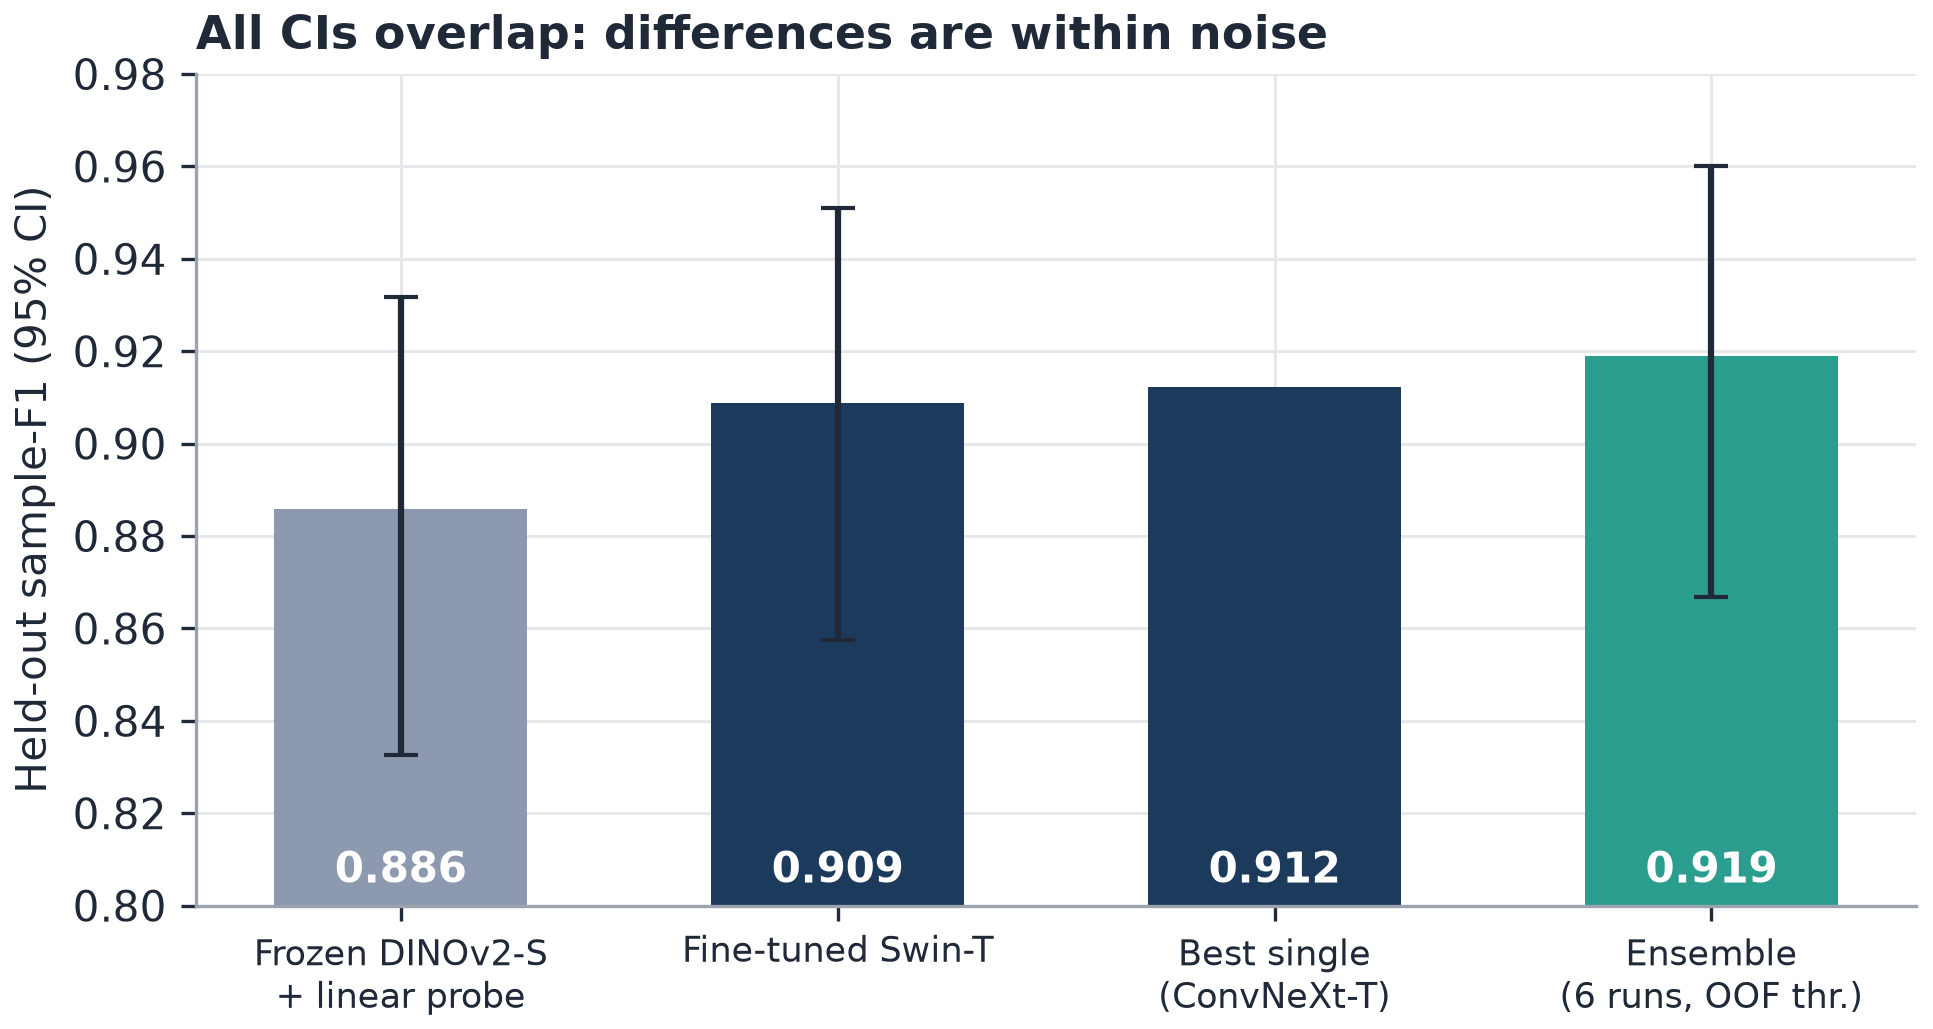
\includegraphics[width=0.8\textwidth]{fig10_heldout_overview.png}\caption{Held-out sample-F1 for a frozen DINOv2-S probe, the fine-tuned Swin-T, the best single model and the ensemble. All 95 \% confidence intervals overlap.}\label{fig:6}\end{figure}\suppressfloats[t]

\subsection{Competition score (Table 3)}
Both late submissions are unranked, and we report every submission we made. The Stage 1 ensemble scored 0.92563 on the private leaderboard and 0.92704 on the public one; the Stage 2 ensemble of 16 models scored 0.92638 and 0.93378. The final private leaderboard has 0.93378 in first place, 0.92787 in second and 0.92488 in third, so both of our submissions would sit between second and third place.

\begin{table}[t]
\centering\small
\caption{Kaggle UNIFESP private score vs. the competition leaderboard}\label{tab:kaggle}
\resizebox{\textwidth}{!}{\begin{tabular}{lcc}
\toprule
\textbf{entry} & \textbf{private\_score} & \textbf{public\_score} \\
\midrule
\#1 Harshit Sheoran & 0.93378 &  \\
\#2 JGK (ResNet50/152, FastAI) & 0.92787 &  \\
ours: stage-2 union (late submission) & 0.92638 & 0.93378 \\
ours: stage-1 ensemble (late submission) & 0.92563 & 0.92704 \\
\#3 Colin Greeley & 0.92488 &  \\
\#4 KobeU Systems Medicine & 0.92414 &  \\
\#5 wangkui & 0.92182 &  \\
\bottomrule
\end{tabular}}
\par\smallskip{\footnotesize Mean F1 (sample-wise); private score uses \textasciitilde{}60 \% of the test set with the original (partly noisy) labels, so differences of \textasciitilde{}0.003 are within noise. Late submissions are not listed on the leaderboard; report ALL submissions made.}
\end{table}


The private score uses about 60 \% of the 743 test images and their original, partly noisy labels. We estimate its standard error at about 0.012, which means the gap to first place (0.0074) cannot be resolved and the gain of Stage 2 over Stage 1 (+0.00075) is indistinguishable from noise.

Stage 2 was evaluated differently, with OOF predictions on all 1,738 training images, so its numbers are not comparable with the held-out results (Table 4). The plain ensemble of 8 models scored 0.9262 [0.9092, 0.9414]. The same models retrained with pseudo-labels from 539 of the 743 unlabelled test images (confidence 0.9 or higher) scored 0.9233 [0.9058, 0.9392], and the union of all 16 models scored 0.9279 [0.9116, 0.9428]. In paired patient-bootstrap comparisons the union beat the plain ensemble by +0.0017 [-0.0010, +0.0046] (p = 0.25), and the pseudo-labelled models fell short of it by 0.0029 [-0.0092, +0.0034] (p = 0.36). Pseudo-labelling on its own did not help. It lowered both OOF F1 and macro-F1 (the latter from 0.8749 to 0.8587). The union's small gain rests on weights fitted to the same OOF predictions, so it is optimistic. The pseudo-labelled set contains no Hand, Hip, Lumbar Spine, Thoracic Spine, Skull, Thigh, Forearm or Clavicles images and 322 Chest images, so it leans heavily towards frequent classes. Because the procedure uses test images, we do not report it as evidence of generalisation.

\setcounter{table}{3}
\begin{table}[!ht]\centering\small
\caption{Stage 2: out-of-fold results on all 1,738 training images and Kaggle late-submission scores}\label{tab:stage2}
\resizebox{\ifdim\width>\textwidth\textwidth\else\width\fi}{!}{\begin{tabular}{p{0.38\textwidth}cccc}
\toprule
\textbf{ensemble} & \textbf{OOF sample-F1 [95\% CI]} & \textbf{macro-F1} & \textbf{subset acc.} & \textbf{Kaggle private / public} \\
\midrule
s2a: 8 models, no pseudo-labels & 0.9262 [0.9092, 0.9414] & 0.8749 & 0.8867 & not submitted \\
s2b: 8 models, pseudo-labels & 0.9233 [0.9058, 0.9392] & 0.8587 & 0.8855 & not submitted \\
s2u: union of s2a and s2b (16 models) & 0.9279 [0.9116, 0.9428] & 0.8754 & 0.8884 & 0.92638 / 0.93378 \\
difference s2u - s2a & +0.0017 [-0.0010, +0.0046], p = 0.25 &  &  &  \\
difference s2b - s2a & -0.0029 [-0.0092, +0.0034], p = 0.36 &  &  &  \\
\bottomrule
\end{tabular}}
\par\smallskip{\footnotesize OOF numbers are not comparable with the held-out numbers of Table 2 (different protocol: no fixed held-out set). Ensemble weights are fitted on the same OOF predictions, so the union estimate is optimistic. CIs: patient-level bootstrap (2,000 resamples); pseudo-labels use unlabelled test images (transductive).}
\end{table}




\subsection{Evaluation shortcuts (Table 5 and Supplementary Table S2)}
With a random image-level split, the validation score exceeded the held-out score by 0.0144; with patient-level folds the difference was 0.0004. The held-out score of the leaky model (0.9163) is not significantly different from the reference (p = 0.141), so leakage distorted the validation estimate rather than the held-out result. Tuning per-class thresholds on the held-out set itself gave 0.9182, against 0.9099 when the thresholds were tuned on OOF predictions (+0.0083). That difference is a gain taken from the test set. Our earlier notebooks, which tuned thresholds and chose checkpoints on the scored fold, reported 0.9356 (sample-F1) and 0.909 (macro-F1). Under the nested protocol the same quantities are 0.9189 and 0.8630 (Fig. 7A).

\begin{figure}[t]\centering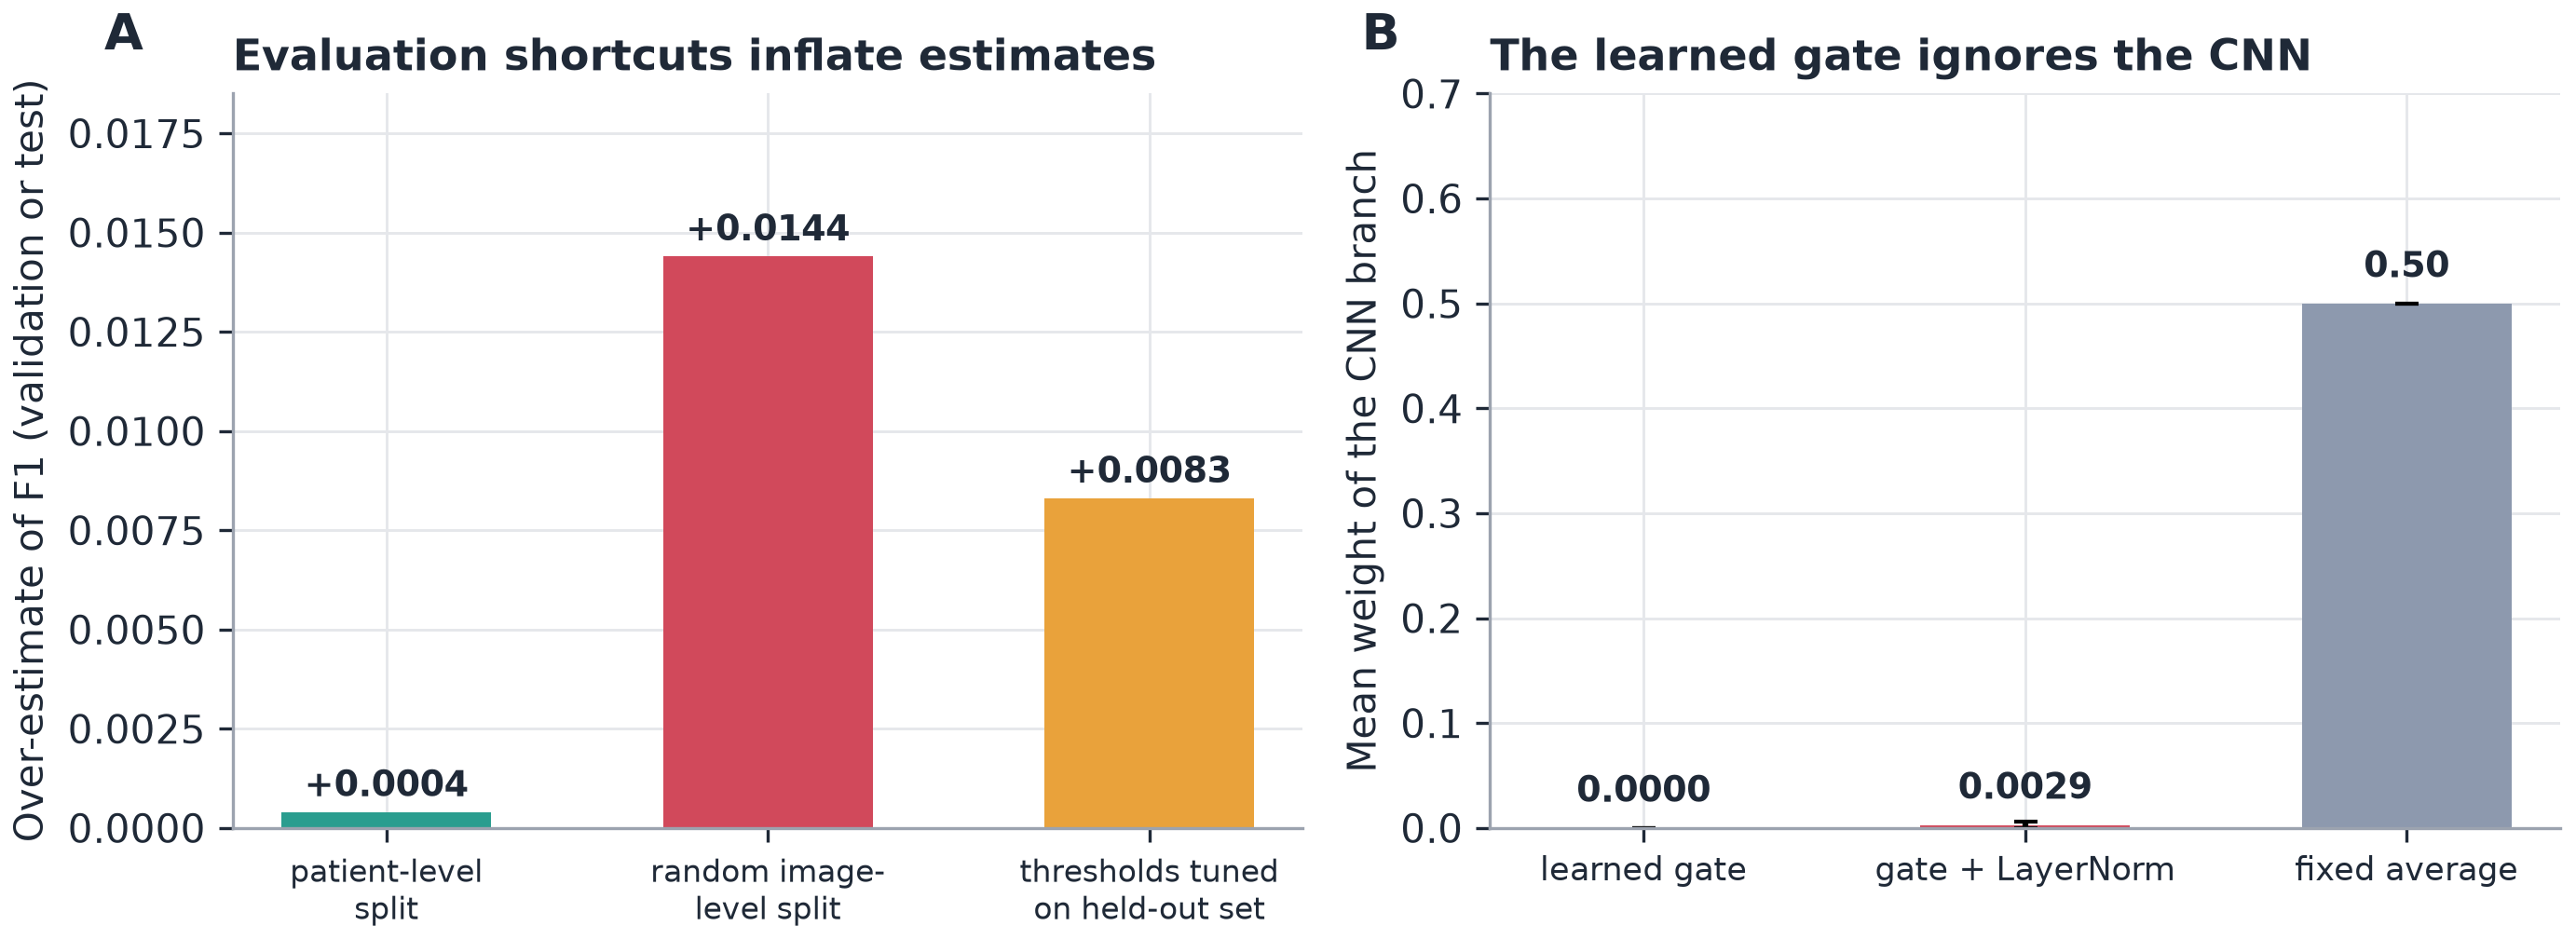
\includegraphics[width=1.0\textwidth]{fig7_leakage_and_gate.png}\caption{(A) How much a random image-level split and tuning thresholds on the held-out set overstate the score. (B) Mean weight the learned fusion gates give the CNN branch, compared with a fixed average.}\label{fig:7}\end{figure}\suppressfloats[t]

\subsection{Ablations (Table 5)}
Against the reference Swin-T (0.9089 [0.8576, 0.9509]) no configuration differed significantly. Heavy augmentation changed F1 by -0.0075 (p = 0.088), dropping the softmax head by -0.0051 (p = 0.152), two other seeds by +0.0055 and +0.0065 (p = 0.37 and 0.27), DenseNet121 by +0.0111 (p = 0.119), the CNN-only fusion branch by +0.0117 (p = 0.097) and the average of three seeds by +0.0049 (p = 0.38). All 95 \% intervals include zero. The seed-to-seed spread (0.9089 to 0.9154) is as large as most of these effects, so a single-run difference of this size should not be called an improvement (Fig. 8).

\setcounter{table}{4}
\begin{table}[!ht]\centering\small
\caption{Ablations (5 CV folds each, same held-out set; paired patient bootstrap vs. the reference)}\label{tab:ablation}
\resizebox{\ifdim\width>\textwidth\textwidth\else\width\fi}{!}{\begin{tabular}{lccccc}
\toprule
\textbf{config} & \textbf{held-out sample-F1 [95\% CI]} & \textbf{macro-F1} & \textbf{OOF - held-out} & \textbf{diff vs reference [95\% CI]} & \textbf{p} \\
\midrule
swin\_tiny\_s224 & 0.9089 [0.8576, 0.9509] & 0.837 & 0.0004 &  &  \\
swin\_tiny\_s224\_heavy & 0.9013 [0.8494, 0.9440] & 0.829 & 0.0074 & -0.0075 [-0.0164, 0.0009] & 0.088 \\
swin\_tiny\_s224\_ce0 & 0.9038 [0.8529, 0.9470] & 0.8261 & 0.0041 & -0.0051 [-0.0124, 0.0016] & 0.152 \\
swin\_tiny\_s224\_ce1 & 0.9132 [0.8616, 0.9568] & 0.8495 & 0.0012 & 0.0043 [-0.0063, 0.0149] & 0.447 \\
swin\_tiny\_s224\_leaky & 0.9163 [0.8644, 0.9587] & 0.856 & 0.0144 & 0.0074 [-0.0020, 0.0178] & 0.141 \\
swin\_tiny\_s224\_seed1 & 0.9143 [0.8620, 0.9576] & 0.8533 & 0.0028 & 0.0055 [-0.0060, 0.0173] & 0.366 \\
swin\_tiny\_s224\_seed2 & 0.9154 [0.8635, 0.9592] & 0.8585 & -0.0014 & 0.0065 [-0.0049, 0.0178] & 0.268 \\
hybrid\_gate\_s224 & 0.9136 [0.8609, 0.9568] & 0.8497 & 0.0000 & 0.0047 [-0.0063, 0.0161] & 0.401 \\
hybrid\_gate\_ln\_s224 & 0.9158 [0.8641, 0.9577] & 0.8536 & -0.0019 & 0.0069 [-0.0032, 0.0182] & 0.226 \\
hybrid\_avg\_s224 & 0.9164 [0.8651, 0.9585] & 0.8537 & -0.0004 & 0.0075 [-0.0048, 0.0201] & 0.235 \\
hybrid\_cnn\_s224 & 0.9205 [0.8684, 0.9613] & 0.8705 & -0.0012 & 0.0117 [-0.0016, 0.0257] & 0.097 \\
hybrid\_swin\_s224 & 0.9127 [0.8611, 0.9565] & 0.8467 & 0.0013 & 0.0038 [-0.0070, 0.0145] & 0.539 \\
densenet121\_s256 & 0.9200 [0.8694, 0.9618] & 0.8542 & -0.0042 & 0.0111 [-0.0022, 0.0275] & 0.119 \\
convnext\_tiny\_s256 & 0.9117 [0.8605, 0.9546] & 0.8472 & 0.0081 & 0.0028 [-0.0084, 0.0142] & 0.674 \\
swin\_3seeds\_average & 0.9137 [0.8623, 0.9574] & 0.848 & 0.0012 & 0.0049 [-0.0052, 0.0148] & 0.38 \\
\bottomrule
\end{tabular}}
\par\smallskip{\footnotesize \texttt{OOF - held-out} large and positive = the validation score over-estimates (compare \texttt{\_leaky} with the patient-level reference for the split ablation).}
\end{table}


\begin{figure}[t]\centering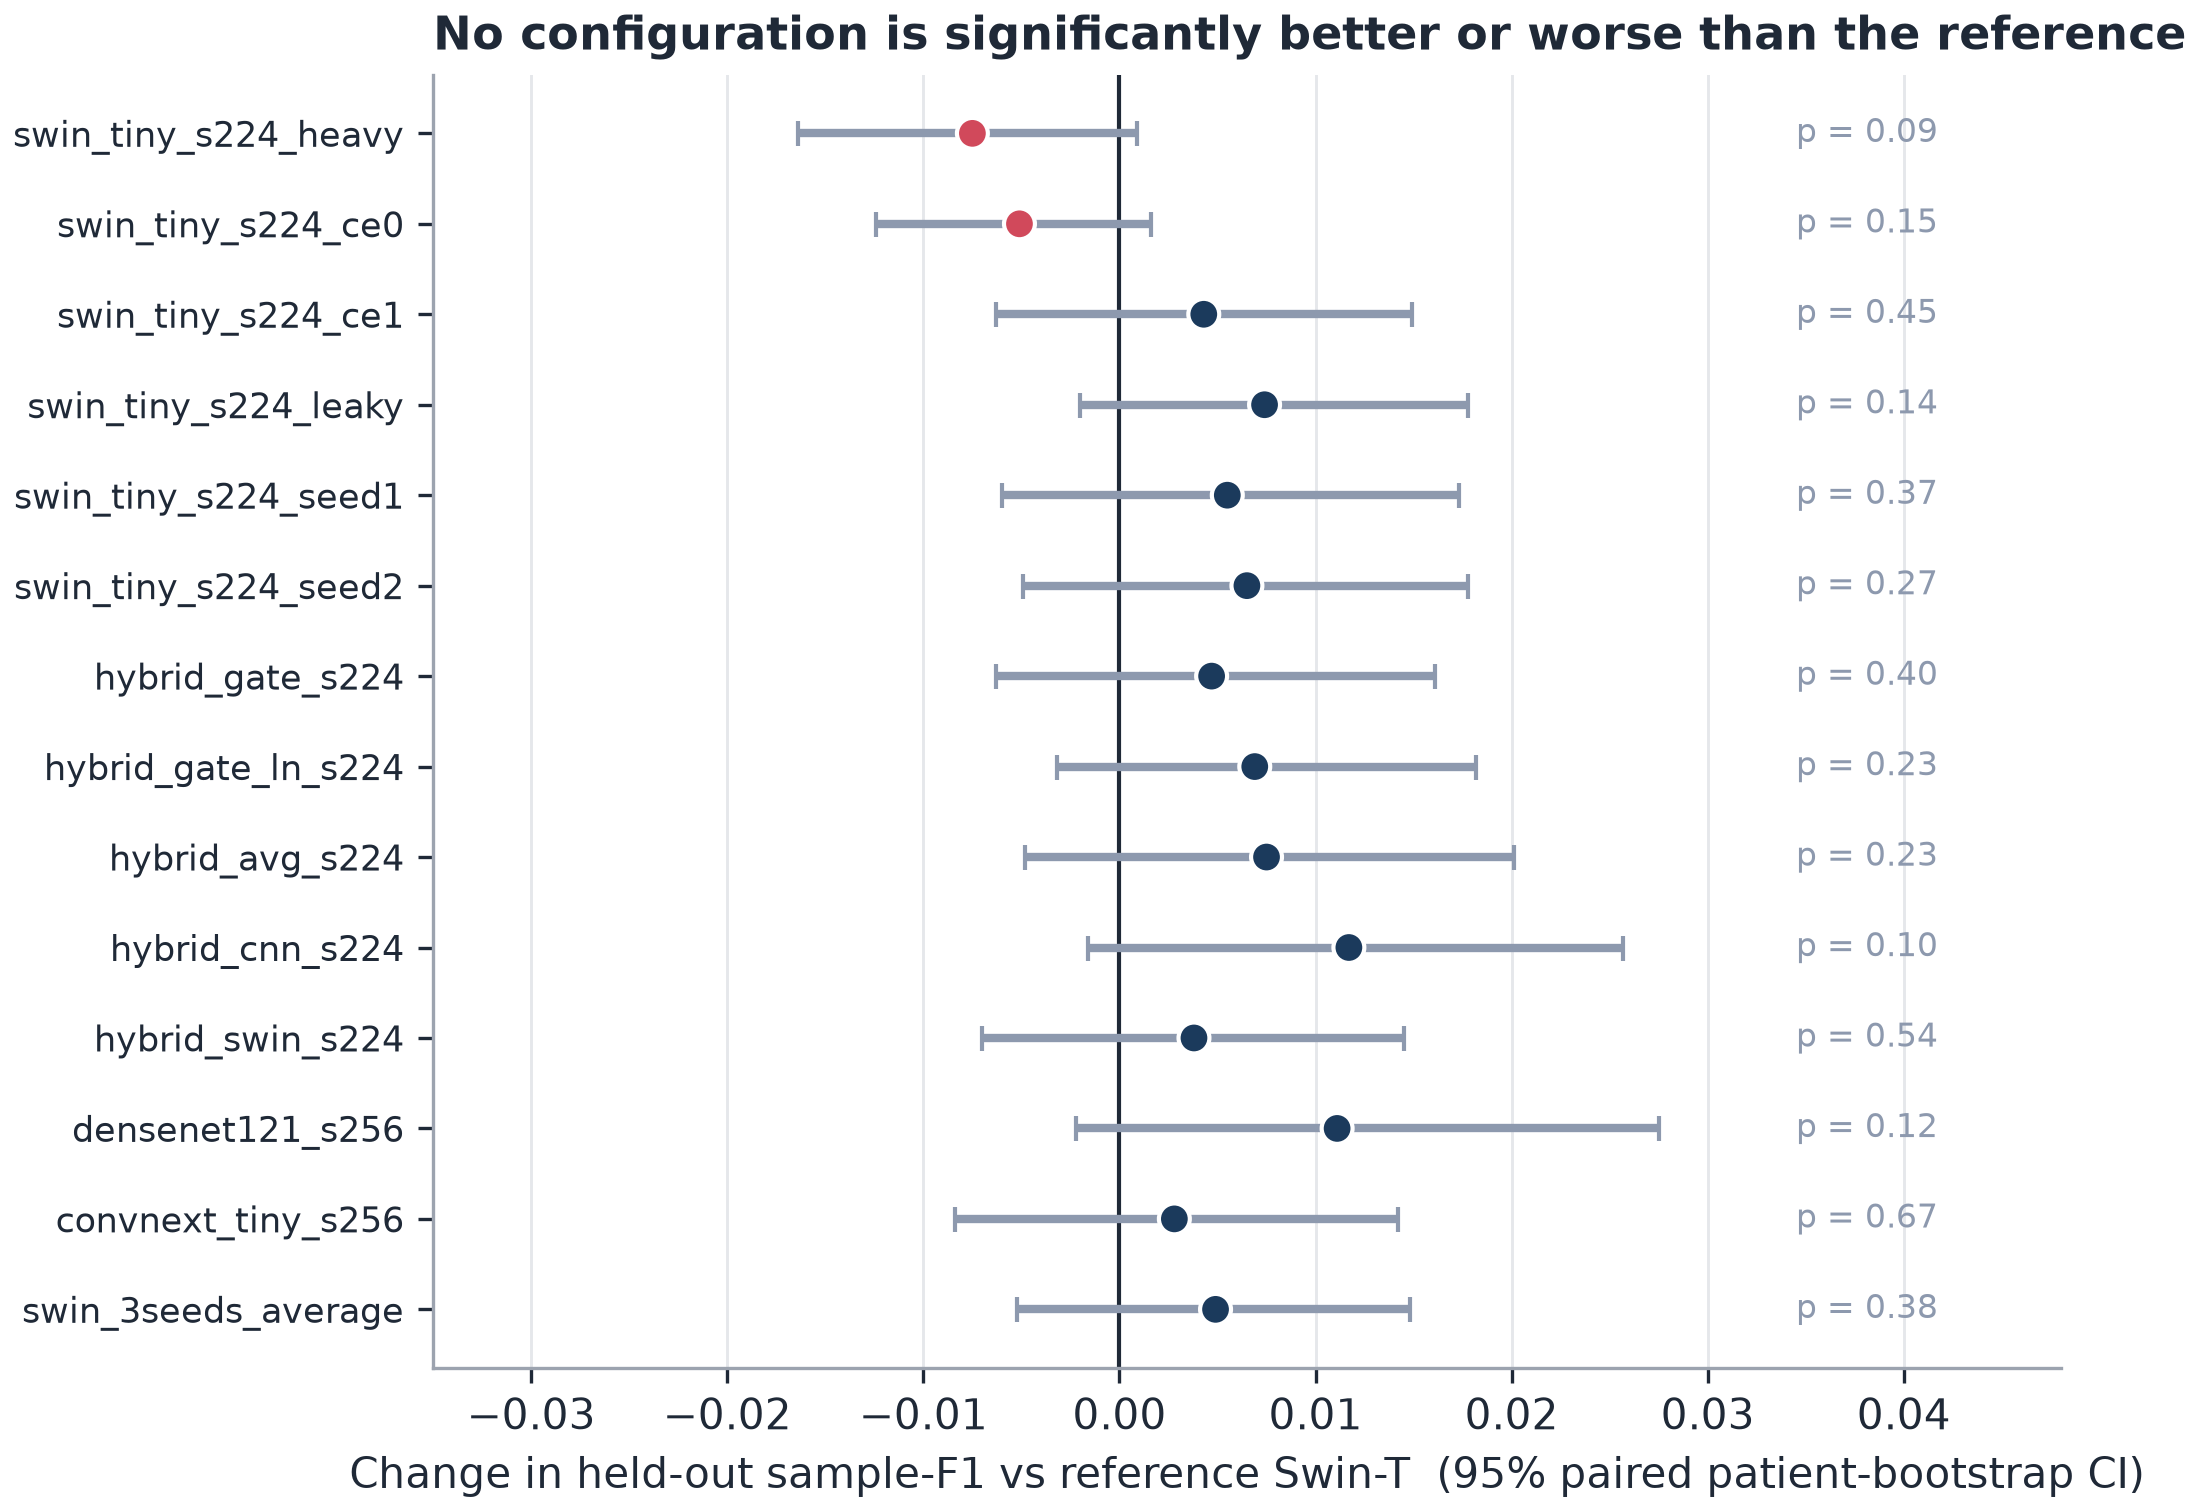
\includegraphics[width=0.9\textwidth]{fig2_ablation_forest.png}\caption{Change in held-out sample-F1 against the reference Swin-T for each ablation (95 \% paired patient-bootstrap interval; p-values on the right). None of the intervals excludes zero.}\label{fig:8}\end{figure}\suppressfloats[t]

\subsection{Fusion gate (Supplementary Table S3)}
Across five folds the learned gate gave the CNN branch a mean weight of 0.0000 (raw gate) and 0.0029 (LayerNorm gate). The fused model therefore behaves like the Transformer alone (Fig. 7B). Neither gate beat the fixed average (+0.0047 and +0.0069 against the reference, p = 0.40 and 0.23) or the CNN-only branch.

\subsection{Frozen foundation-model baseline}
A linear probe on frozen DINOv2-S reached 0.8699 OOF and 0.8859 on the held-out set [0.8327, 0.9318]. DINOv2-B reached 0.8839 [0.8300, 0.9276] and the ImageNet Swin-T 0.8762 [0.8248, 0.9204], while the fine-tuned Swin-T reference reached 0.9089. Frozen features therefore recover most of the fine-tuned performance, but not all of it. With 10 \% of the training patients the DINOv2-S probe scored 0.6435 OOF, with 25 \% 0.7457, with 50 \% 0.8235 and with all of them 0.8699. The curve is still rising, so this task looks limited by labelled data. A random-weight ResNet18 control gave 0.563 OOF but 0.095 on the held-out set, an inconsistency we could not resolve, so we leave it out of our claims. BiomedCLIP could not be downloaded and one ConvNeXt tag was invalid; both were skipped (Fig. 9).

\begin{figure}[t]\centering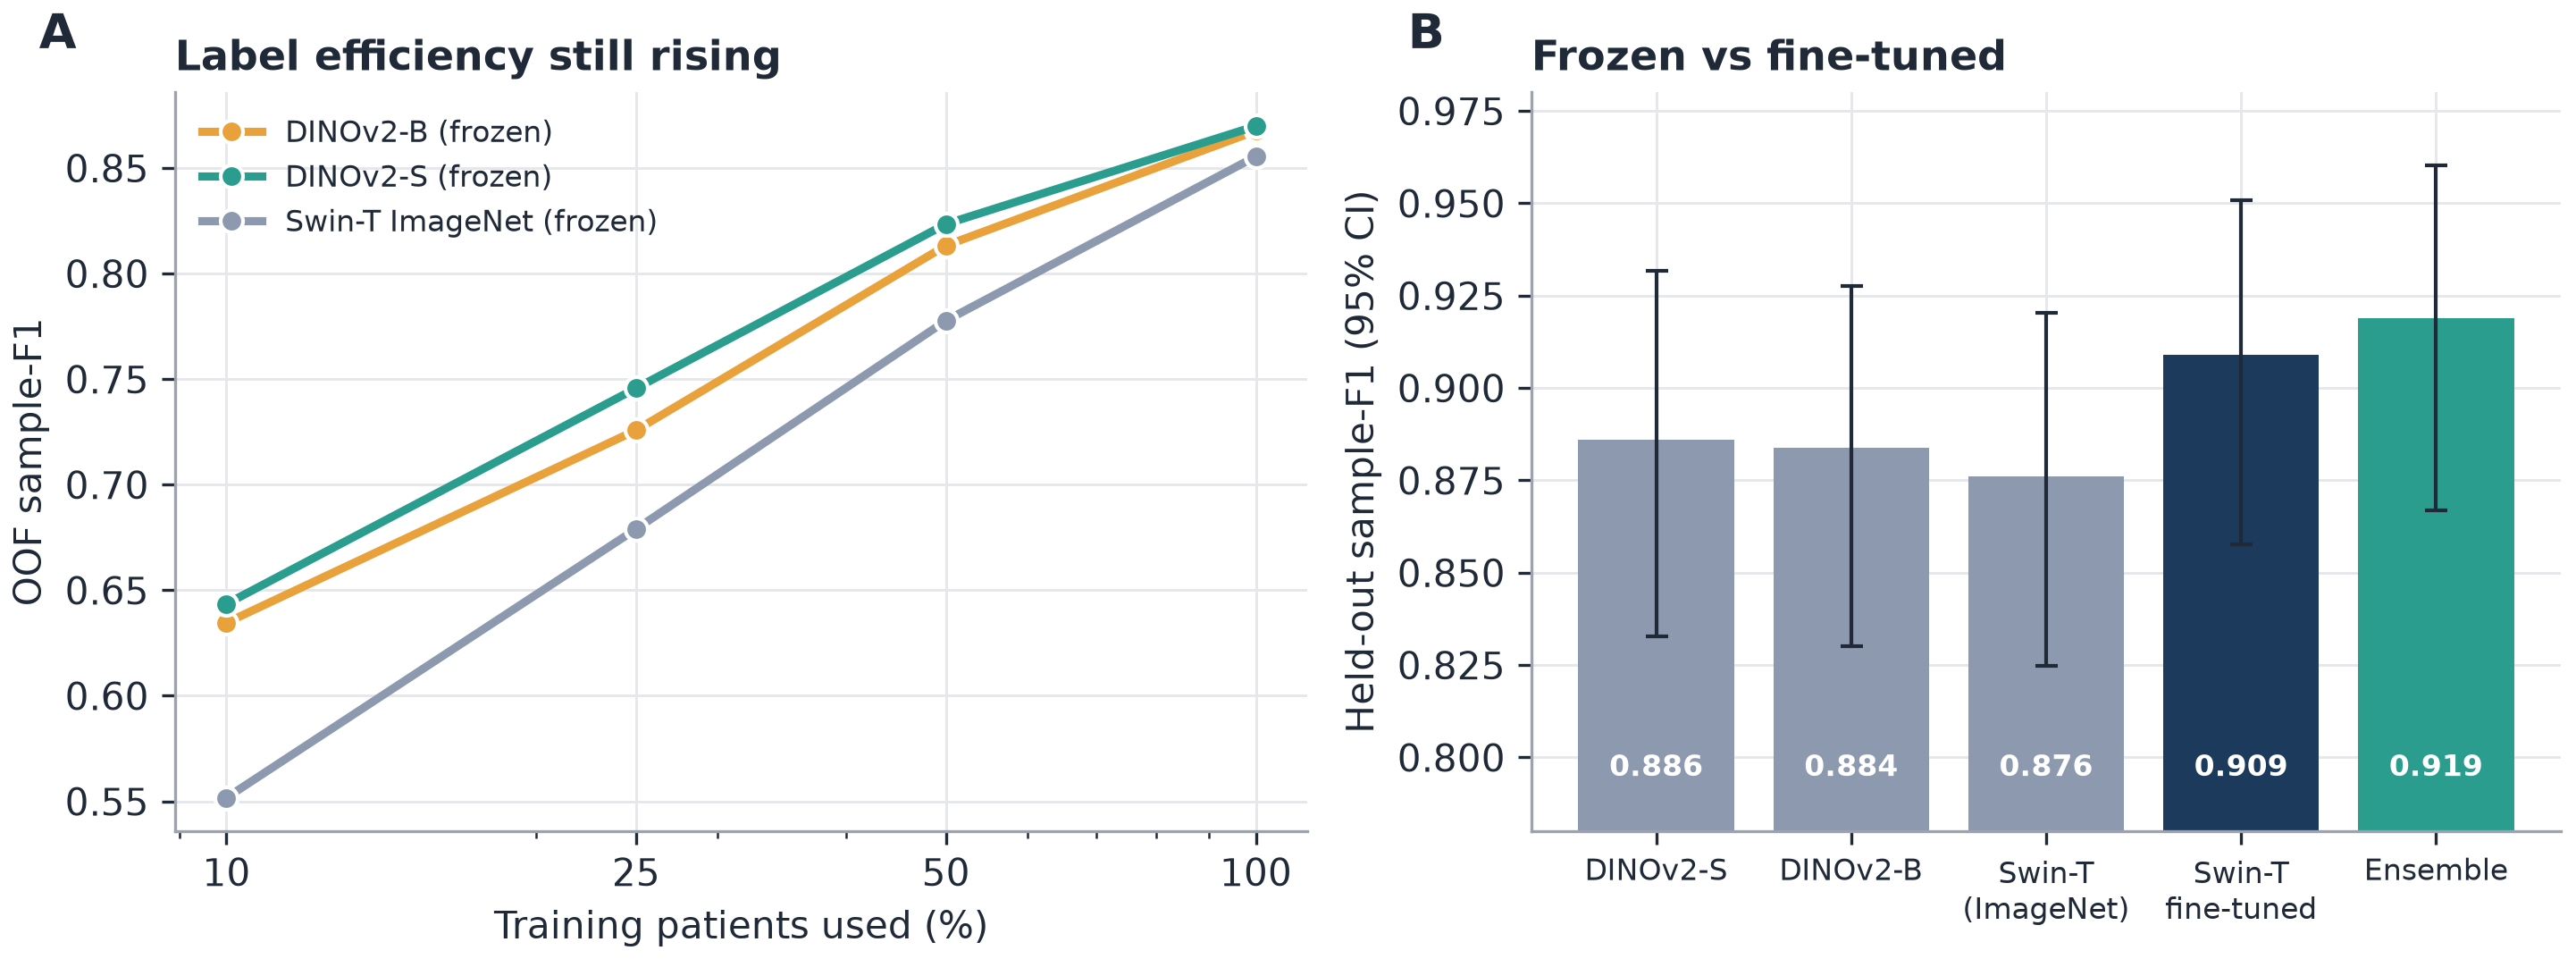
\includegraphics[width=1.0\textwidth]{fig5_foundation_models.png}\caption{(A) Label efficiency of frozen encoders. (B) Held-out F1 of the frozen probes next to the fine-tuned models.}\label{fig:9}\end{figure}\suppressfloats[t]

\subsection{Reliability and label audit}
\textbf{Calibration.} Top-1 accuracy of the five-model ensemble on the held-out set was 0.9257. ECE was 0.0545, and 0.0517 after temperature scaling (T = 1.15), so the ensemble is already close to calibrated and scaling changes little.

\textbf{Selective prediction.} Accuracy on the images the model kept rose from 0.926 at full coverage to 0.945 [0.900, 0.985] at 90 \% coverage, 0.973 at 80 \% and 0.982 at 70 \%. A threshold chosen on OOF predictions for 0.95 accuracy gave 0.937 accuracy at 98.5 \% coverage on the held-out set, so the target was missed. A 0.98 target gave 0.983 at 74 \% coverage. Operating points chosen on OOF predictions therefore do not transfer exactly (Fig. 10).


\textbf{Per class (held-out).} Chest reached an F1 of 0.993 (n = 138), and Cervical Spine, Feet, Hand, Sinus, Skull and Thigh reached 1.0. The weakest classes were Others (recall 0.41 [0.13, 0.91]), Forearm (0.33), Hip (0.33), Shoulder (0.60) and Ankle (0.75), all with 3 to 22 positives and wide intervals (Supplementary Table S7 and Supplementary Fig. S1).

\begin{figure}[t]\centering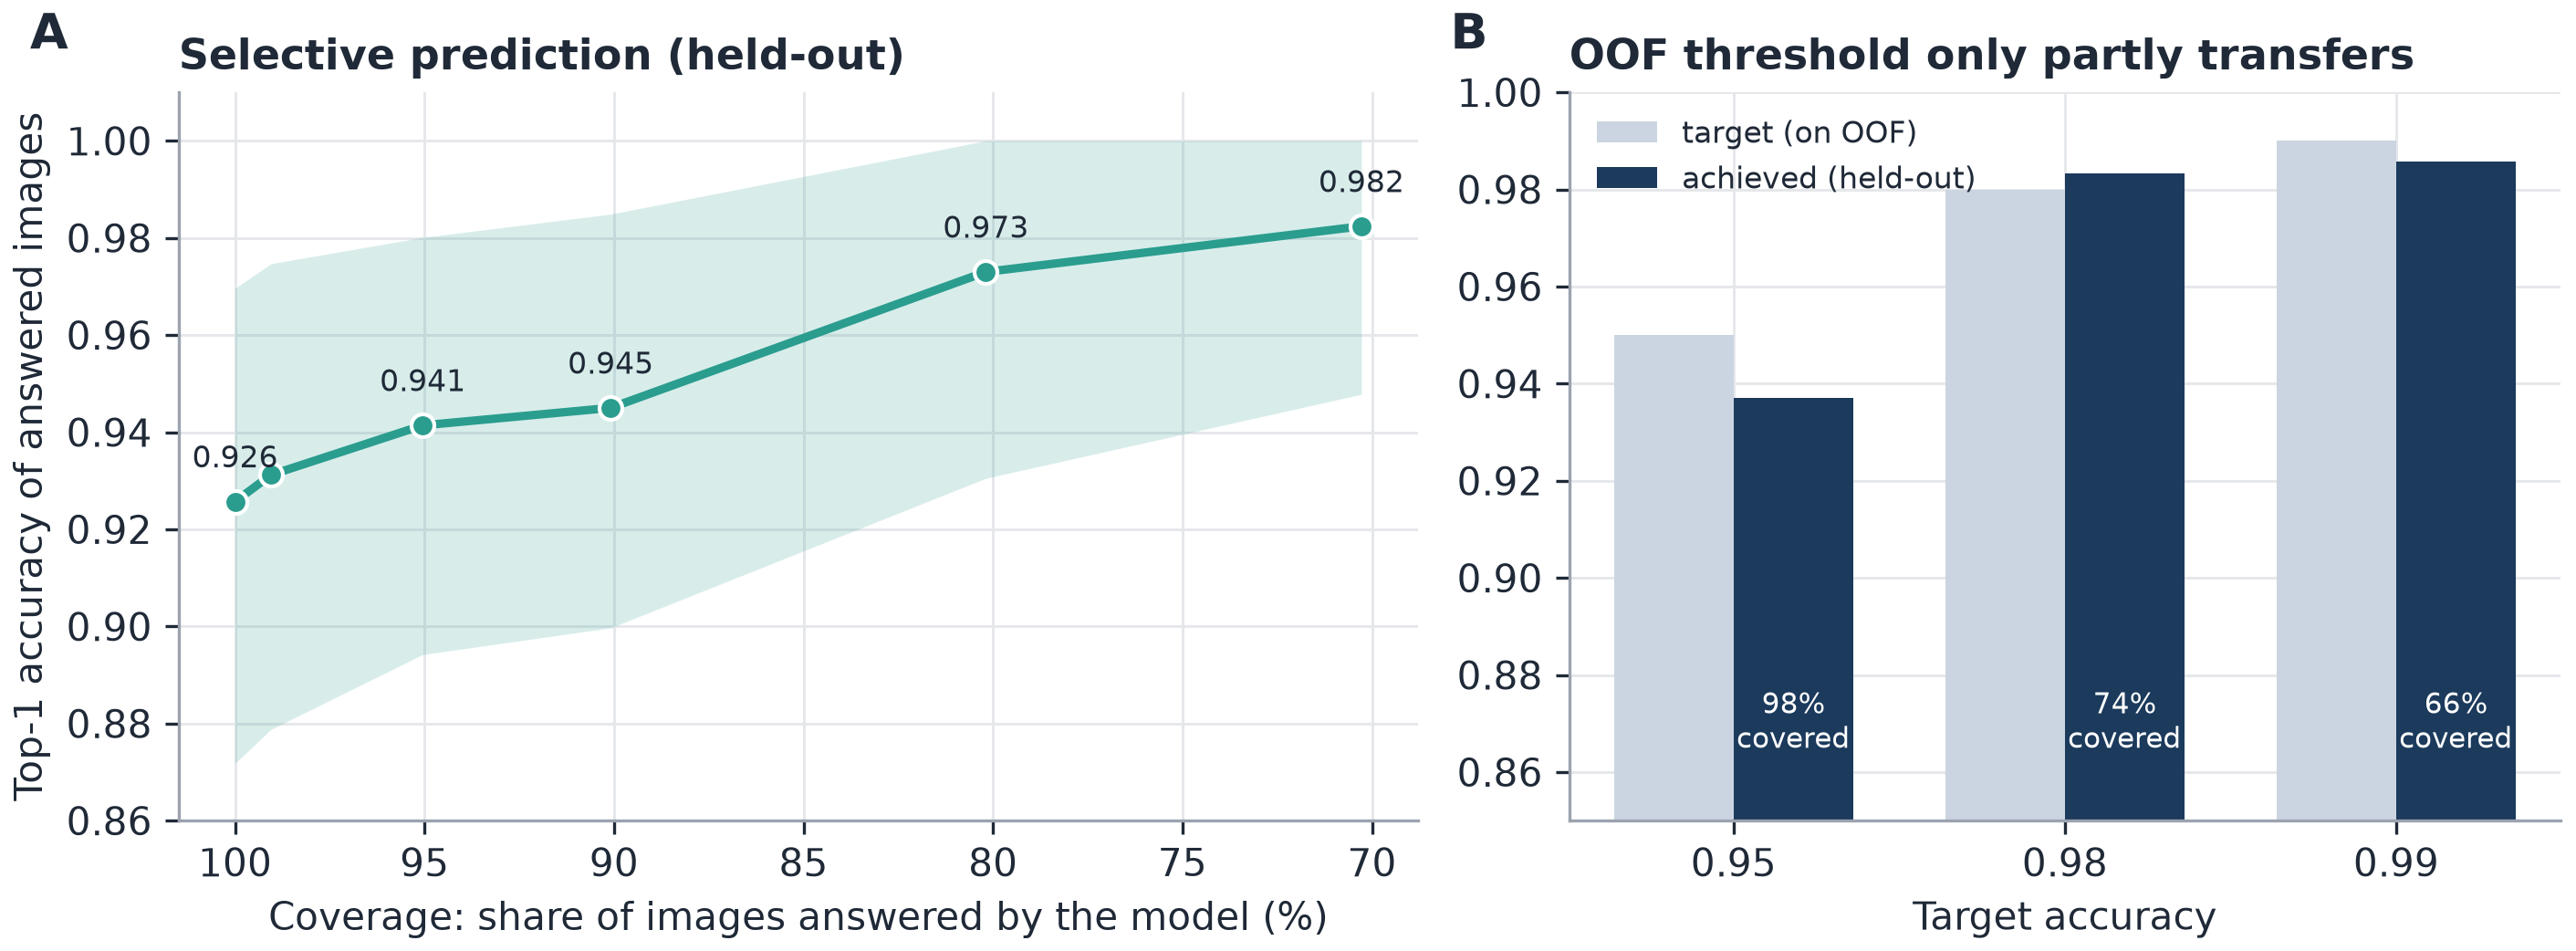
\includegraphics[width=0.8\textwidth]{fig4_reliability.png}\caption{(A) Accuracy on the images the model answers, as a function of coverage. (B) Accuracy targets chosen on out-of-fold predictions, and the accuracy reached on the held-out set.}\label{fig:10}\end{figure}\suppressfloats[t]



\begin{figure}[t]\centering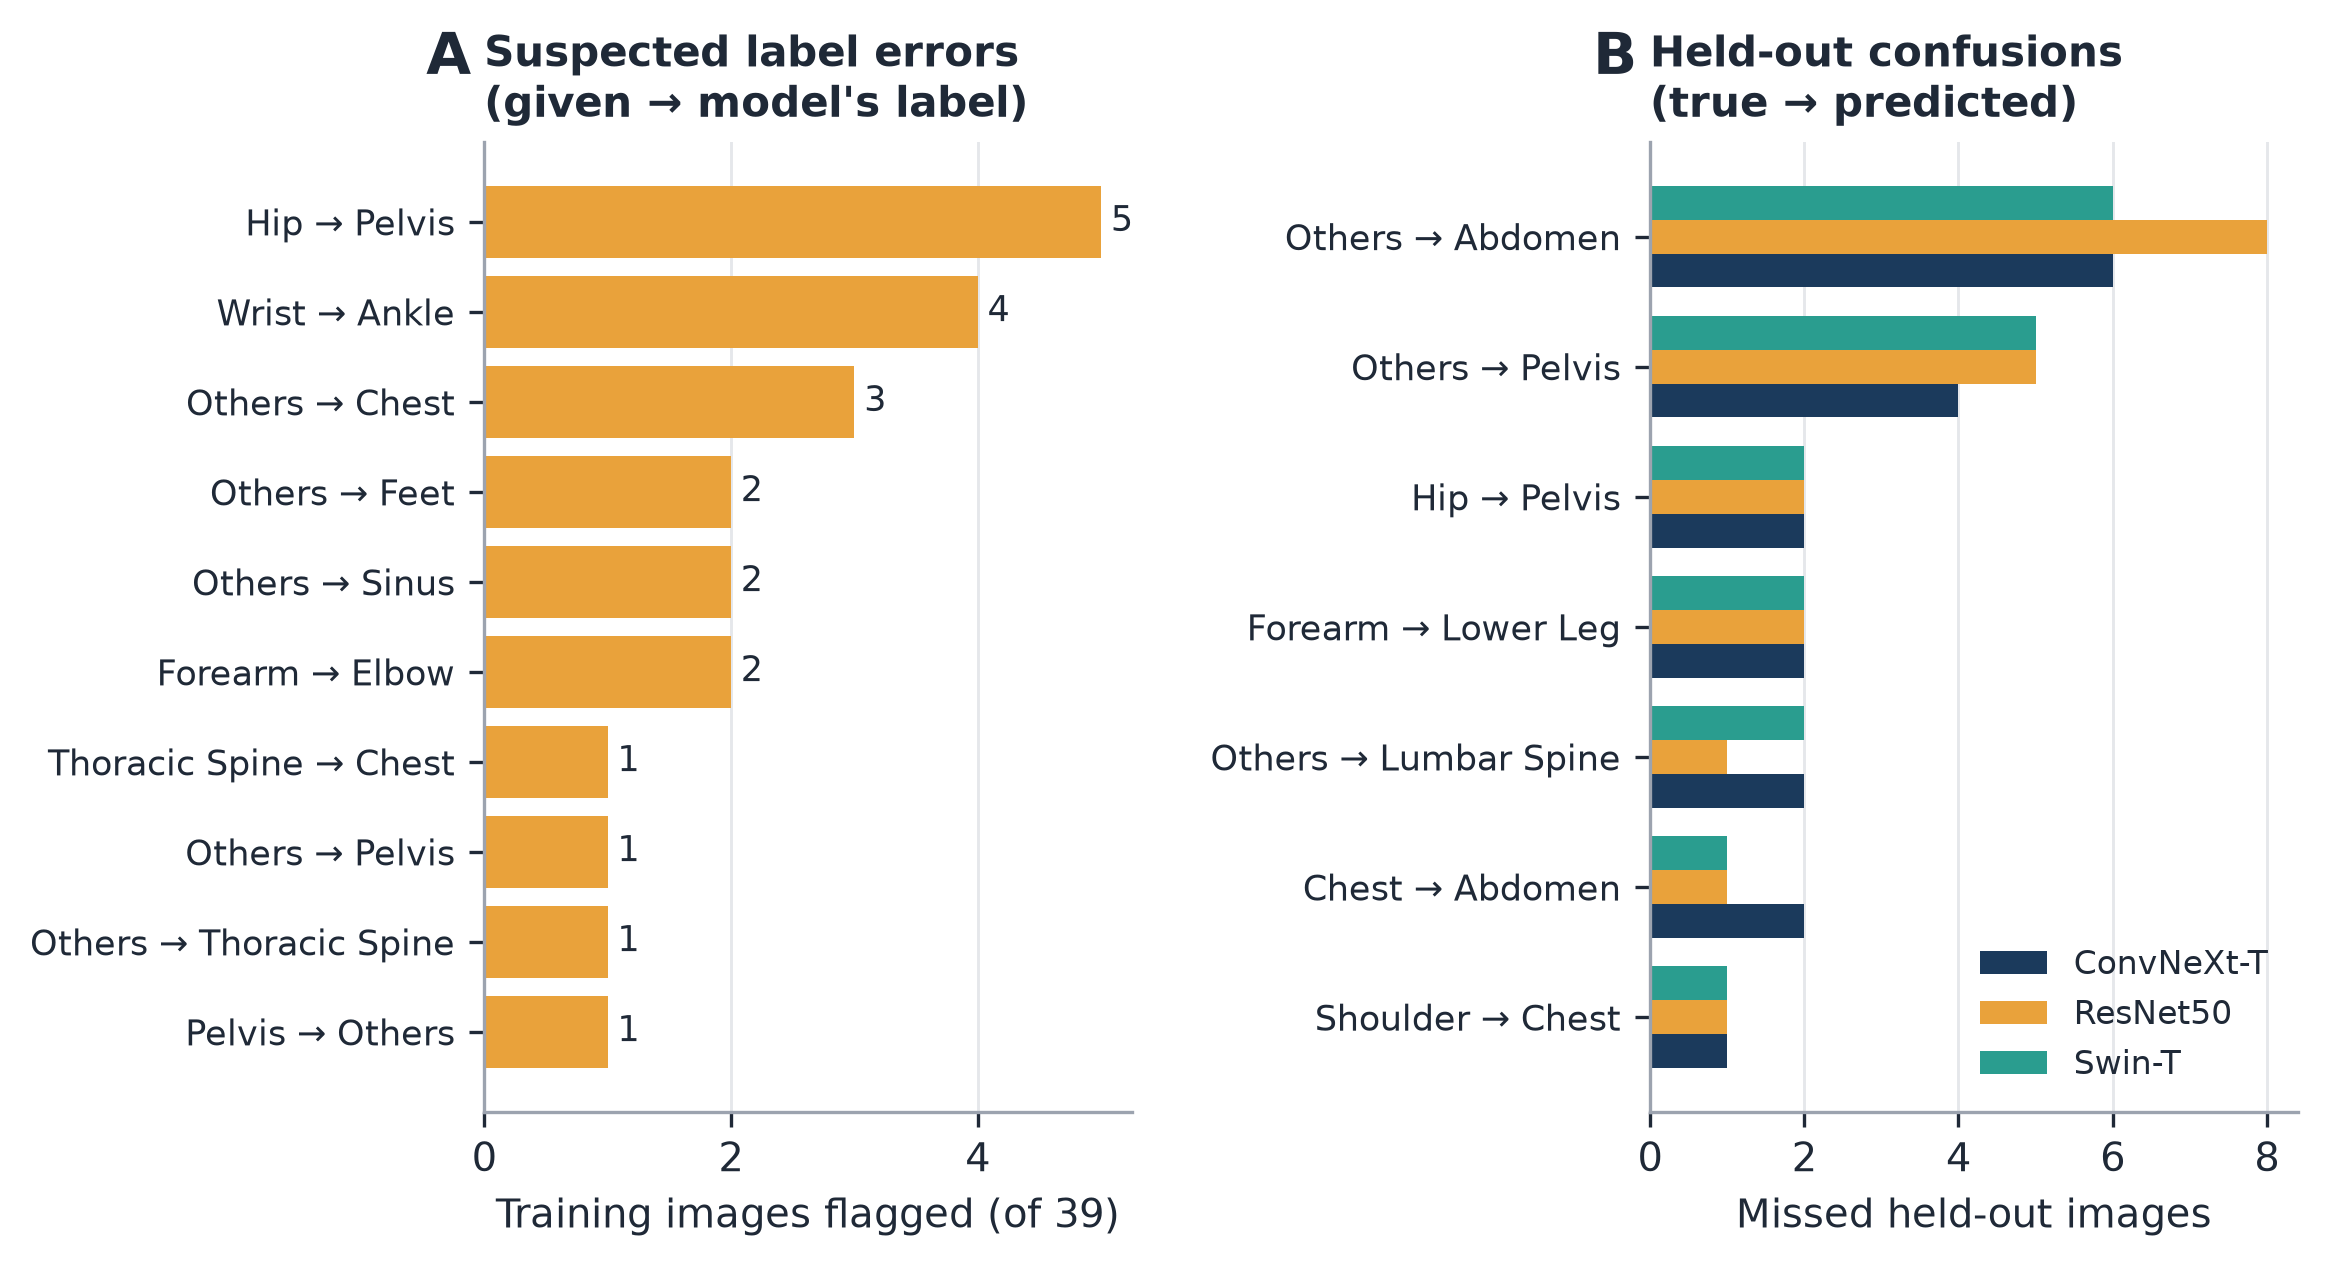
\includegraphics[width=1.0\textwidth]{c2_audit_confusions.png}\caption{(A) The pairs of given and suggested labels among the 39 suspected label errors. (B) The most frequent misclassifications of the three explained models on the held-out set.}\label{fig:11}\end{figure}\suppressfloats[t]
\textbf{Label audit.} At p of 0.9 or more, 39 of 1,415 training images (2.8 \%) were flagged. The most frequent pairs were Hip to Pelvis (5), Wrist to Ankle (4) and Others to Chest (3). The Hip-to-Pelvis pattern mirrors the low Hip recall, which fits either label noise or a real boundary problem between the two classes. No clinician has reviewed any of the 39 suspects.


\textbf{Error analysis (Supplementary Table S6).} In the three explained fold-0 models the most frequent held-out misses were Others labelled as Abdomen (6 to 8 images per model) and Others labelled as Pelvis (4 to 5), followed by Hip as Pelvis (2 per model) and Forearm as Lower Leg (2 per model). The heterogeneous "Others" class is mostly absorbed by large body regions. Fig. 11 shows which label pairs the suspects fall into (A) and how the three explained models misclassify the held-out images (B).



\subsection{Generalisation (Table 6 and Table 7; Supplementary Table S4)}
On the official MURA split the five-fold bagged ensemble reached an accuracy of 0.9747 [0.9663, 0.9818] and a macro-F1 of 0.9707 [0.9616, 0.9788]. Shah et al. (2026) report 0.9643 and 0.9574 on the same 3,197-image validation set, so the two results are comparable in data but not in method details.

On COVID-19 Radiography (4 classes, image-level split) sample-F1 was 0.9647 [0.9595, 0.9697] and macro-F1 0.9681, and these numbers may be optimistic.

Zero-shot transfer (Table 7) gave 0.875 to 0.880 from MURA to UNIFESP (n = 184) and 0.813 to 0.821 from UNIFESP to MURA (n = 12,000). From MURA to FracAtlas, restricted to hand and shoulder (1,281 of the 1,382 images are hand), accuracy was 0.691 with the softmax head and 0.858 with the sigmoid head. From UNIFESP to FracAtlas (hand, hip, leg, shoulder; n = 3,685) it was 0.708 and 0.698. Many FracAtlas JPEGs are truncated and were decoded only partly. Fig. 12 summarises the MURA comparison (A) and the transfer results (B).

\setcounter{table}{4}
\begin{table}[!ht]\centering\small
\caption{MURA body-part classification: held-out = MURA validation set}\label{tab:mura}
\resizebox{\textwidth}{!}{\begin{tabular}{lcc}
\toprule
\textbf{model} & \textbf{accuracy [95\% CI]} & \textbf{macro-F1 [95\% CI]} \\
\midrule
ours: 5-fold bagged ensemble (official MURA split) & 0.9747 [0.9663, 0.9818] & 0.9707 [0.9616, 0.9788] \\
Xception-Swin (Shah 2026) & 0.9643 (CI n/a) & 0.9574 (CI n/a) \\
DenseNet-201 & 0.9187 (CI n/a) & 0.9093 (CI n/a) \\
EfficientNet-B0 & 0.9043 (CI n/a) & 0.8952 (CI n/a) \\
ResNet-101 & 0.8934 (CI n/a) & 0.8831 (CI n/a) \\
VGG-19 & 0.8612 (CI n/a) & 0.8498 (CI n/a) \\
\bottomrule
\end{tabular}}
\par\smallskip{\footnotesize Shah et al. 2026 (Supplementary Table S4; verified in the full text): same MURA validation set (3,197 images), fixed seed 42, image-level evaluation; no CI is shown for these body-part numbers.}
\end{table}


\setcounter{table}{6}
\begin{table}[!ht]\centering\small
\caption{Zero-shot cross-dataset transfer through the class map}\label{tab:transfer}
\resizebox{\ifdim\width>\textwidth\textwidth\else\width\fi}{!}{\begin{tabular}{lccccccc}
\toprule
\textbf{source} & \textbf{target} & \textbf{head} & \textbf{groups} & \textbf{n} & \textbf{accuracy} & \textbf{95 \% CI} & \textbf{macro-F1} \\
\midrule
mura & unifesp & softmax & elbow,finger,forearm,hand,shoulder,wrist & 184 & 0.875 & [0.826, 0.924] & 0.8478 \\
mura & unifesp & sigmoid & elbow,finger,forearm,hand,shoulder,wrist & 184 & 0.8804 & [0.837, 0.924] & 0.856 \\
unifesp & mura & softmax & elbow,finger,forearm,hand,shoulder,wrist & 12000 & 0.8133 & [0.806, 0.820] & 0.7444 \\
unifesp & mura & sigmoid & elbow,finger,forearm,hand,shoulder,wrist & 12000 & 0.8208 & [0.814, 0.828] & 0.7481 \\
mura & fracatlas & softmax & hand,shoulder & 1382 & 0.691 & [0.667, 0.715] & 0.5606 \\
mura & fracatlas & sigmoid & hand,shoulder & 1382 & 0.8575 & [0.840, 0.875] & 0.7115 \\
unifesp & fracatlas & softmax & hand,hip,leg,shoulder & 3685 & 0.708 & [0.693, 0.722] & 0.7409 \\
unifesp & fracatlas & sigmoid & hand,hip,leg,shoulder & 3685 & 0.6982 & [0.684, 0.713] & 0.699 \\
\bottomrule
\end{tabular}}
\par\smallskip{\footnotesize Closed-set decision among the shared groups; CIs are image-level (the targets have no patient ids). The class map is an assumption to be checked by a clinician.}
\end{table}


\begin{figure}[t]\centering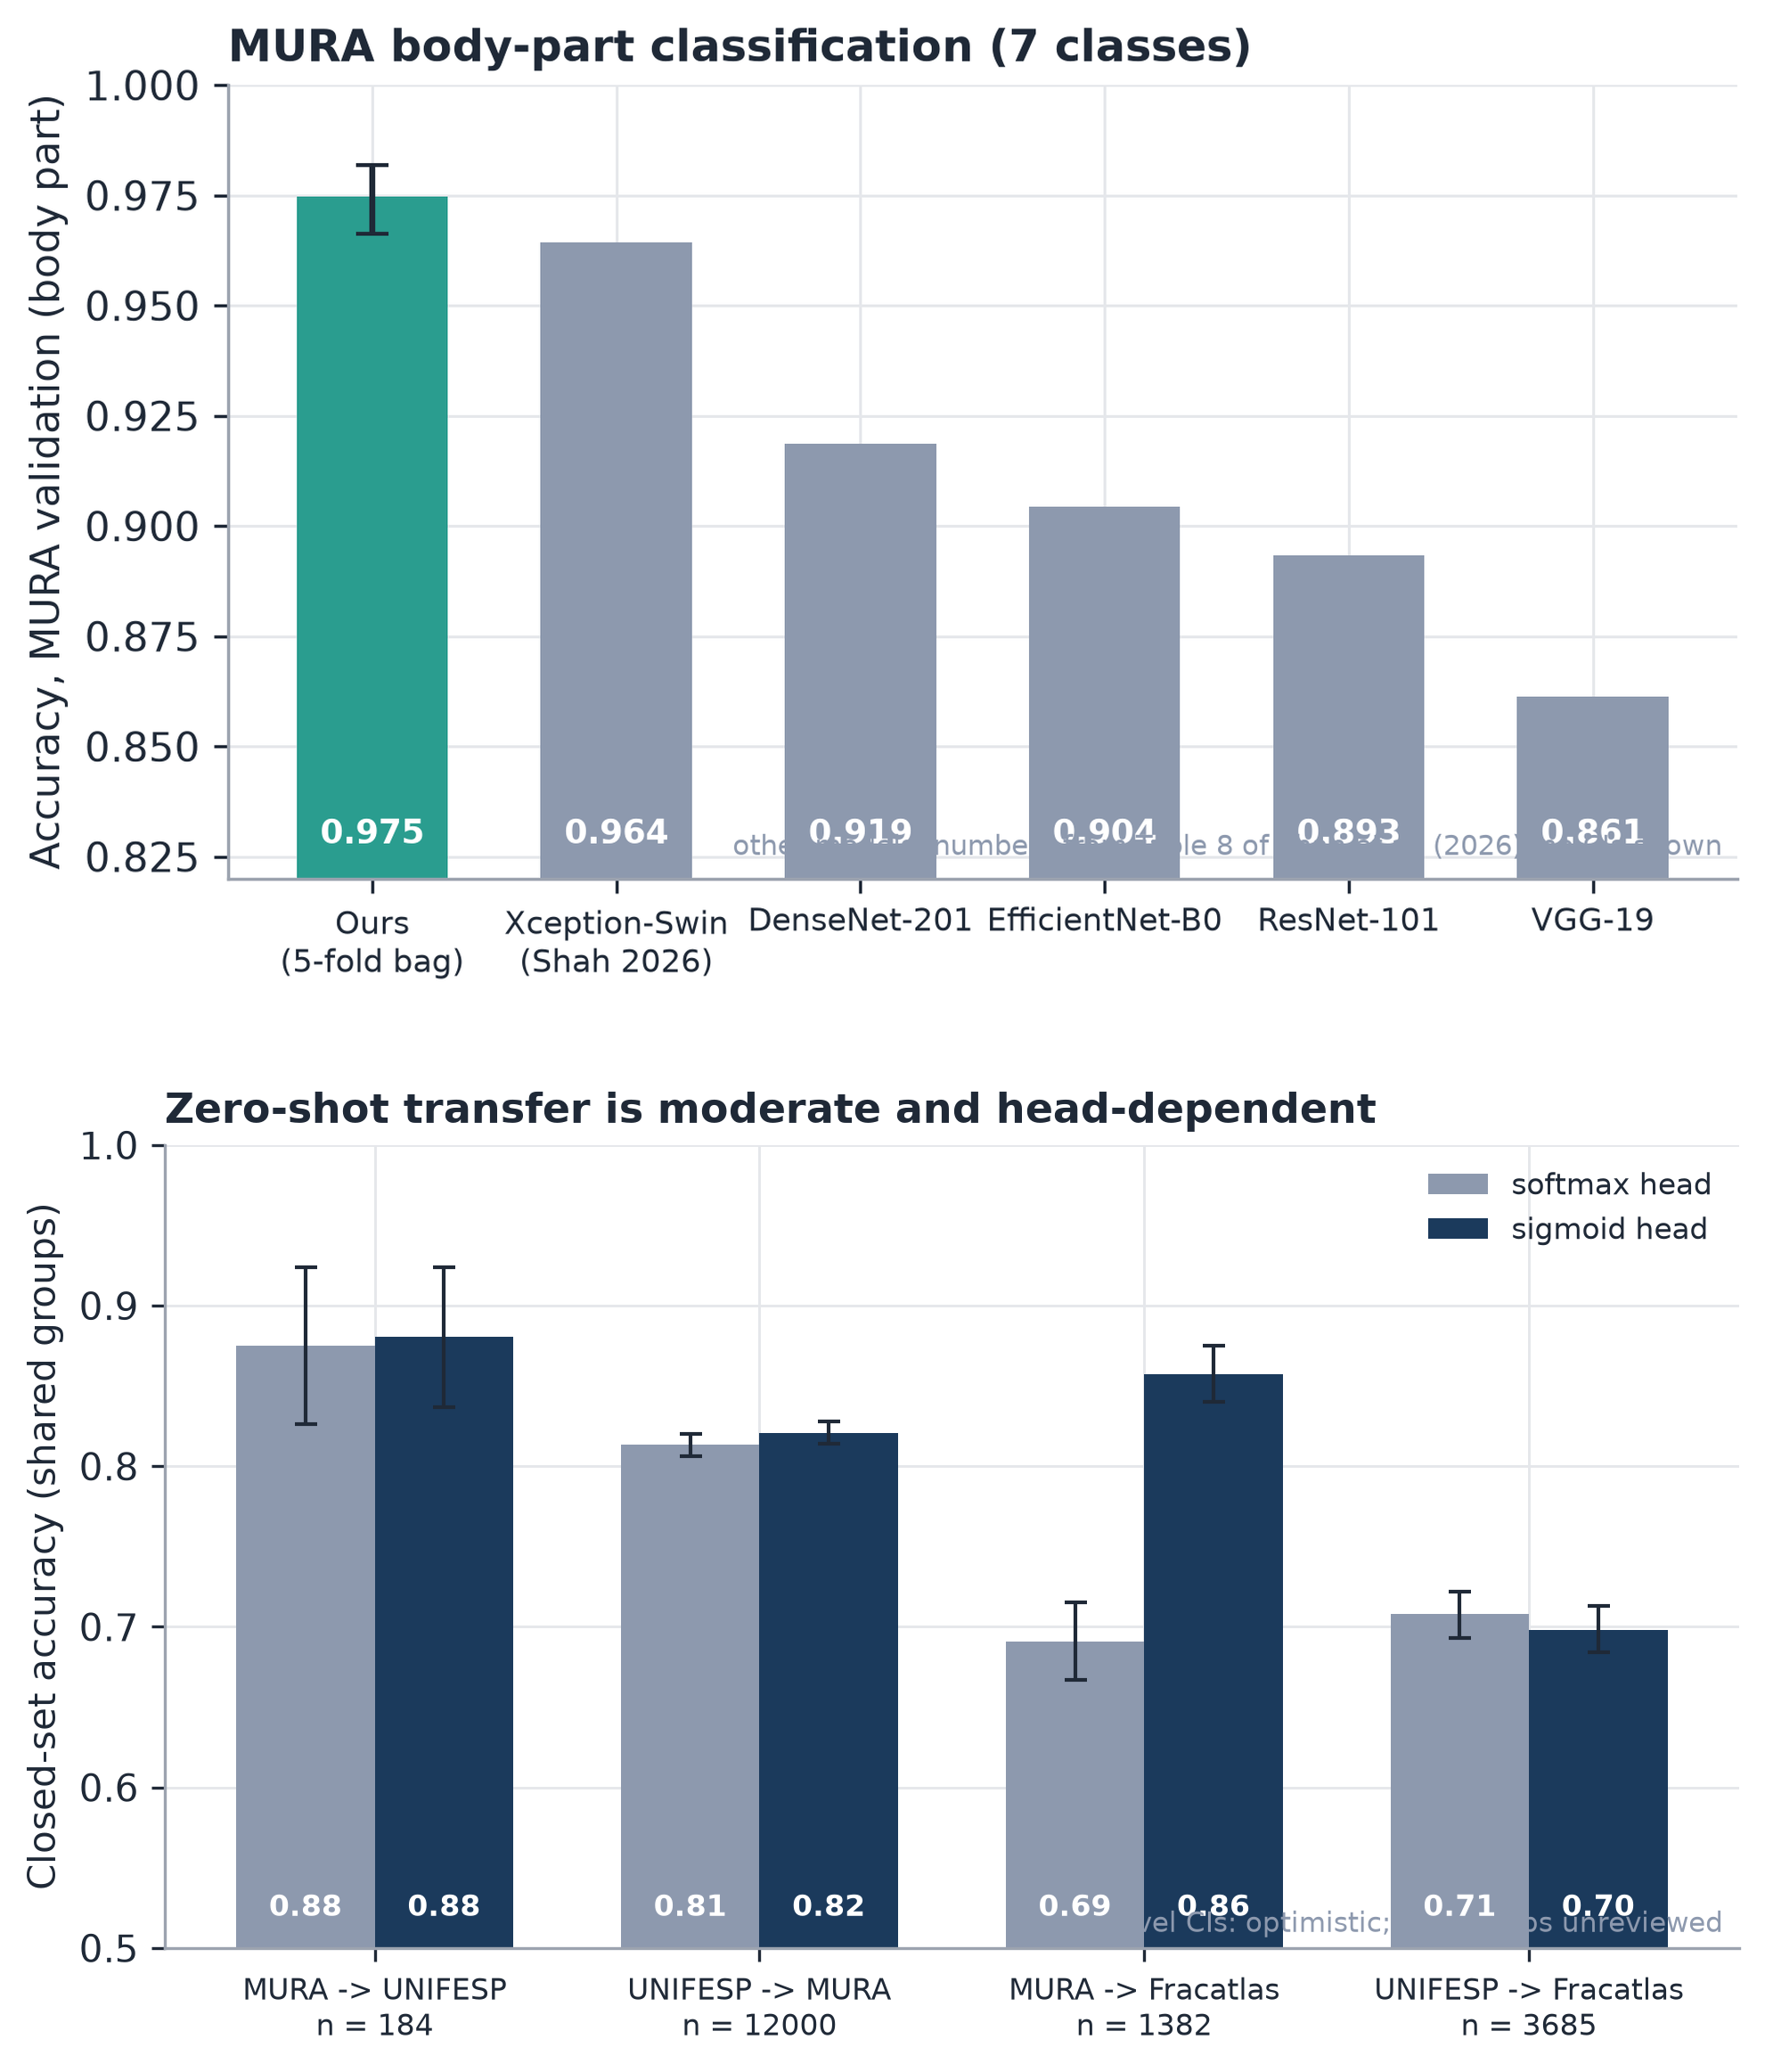
\includegraphics[width=1.0\textwidth]{c3_mura_transfer.png}\caption{(A) Body-part accuracy on MURA (seven classes), compared with the models reported by Shah et al. (2026). (B) Zero-shot accuracy through the class map, for the softmax and sigmoid heads; intervals come from an image-level bootstrap and are optimistic.}\label{fig:12}\end{figure}\suppressfloats[t]
Transfer is moderate and depends on the head, and the class maps are our own assumptions.


\subsection{Explainability (Supplementary Table S5)}
For all three models, deleting the most salient pixels first removed class evidence faster than deleting a random block of the same size (gain 0.284 [0.252, 0.316] for ConvNeXt-T, 0.204 for ResNet50, 0.164 for Swin-T). The maps were uncorrelated with those of randomly initialised networks for ConvNeXt-T and Swin-T (rho 0.11 and 0.02). ResNet50 differed too, but with a systematic negative correlation (rho -0.31). The feature grids are coarse (7 $\times$ 7 to 8 $\times$ 8), there is no localisation ground truth and no radiologist reviewed the maps. We therefore describe them as faithful to the model, not as clinically valid (Fig. 13).

\begin{figure}[t]\centering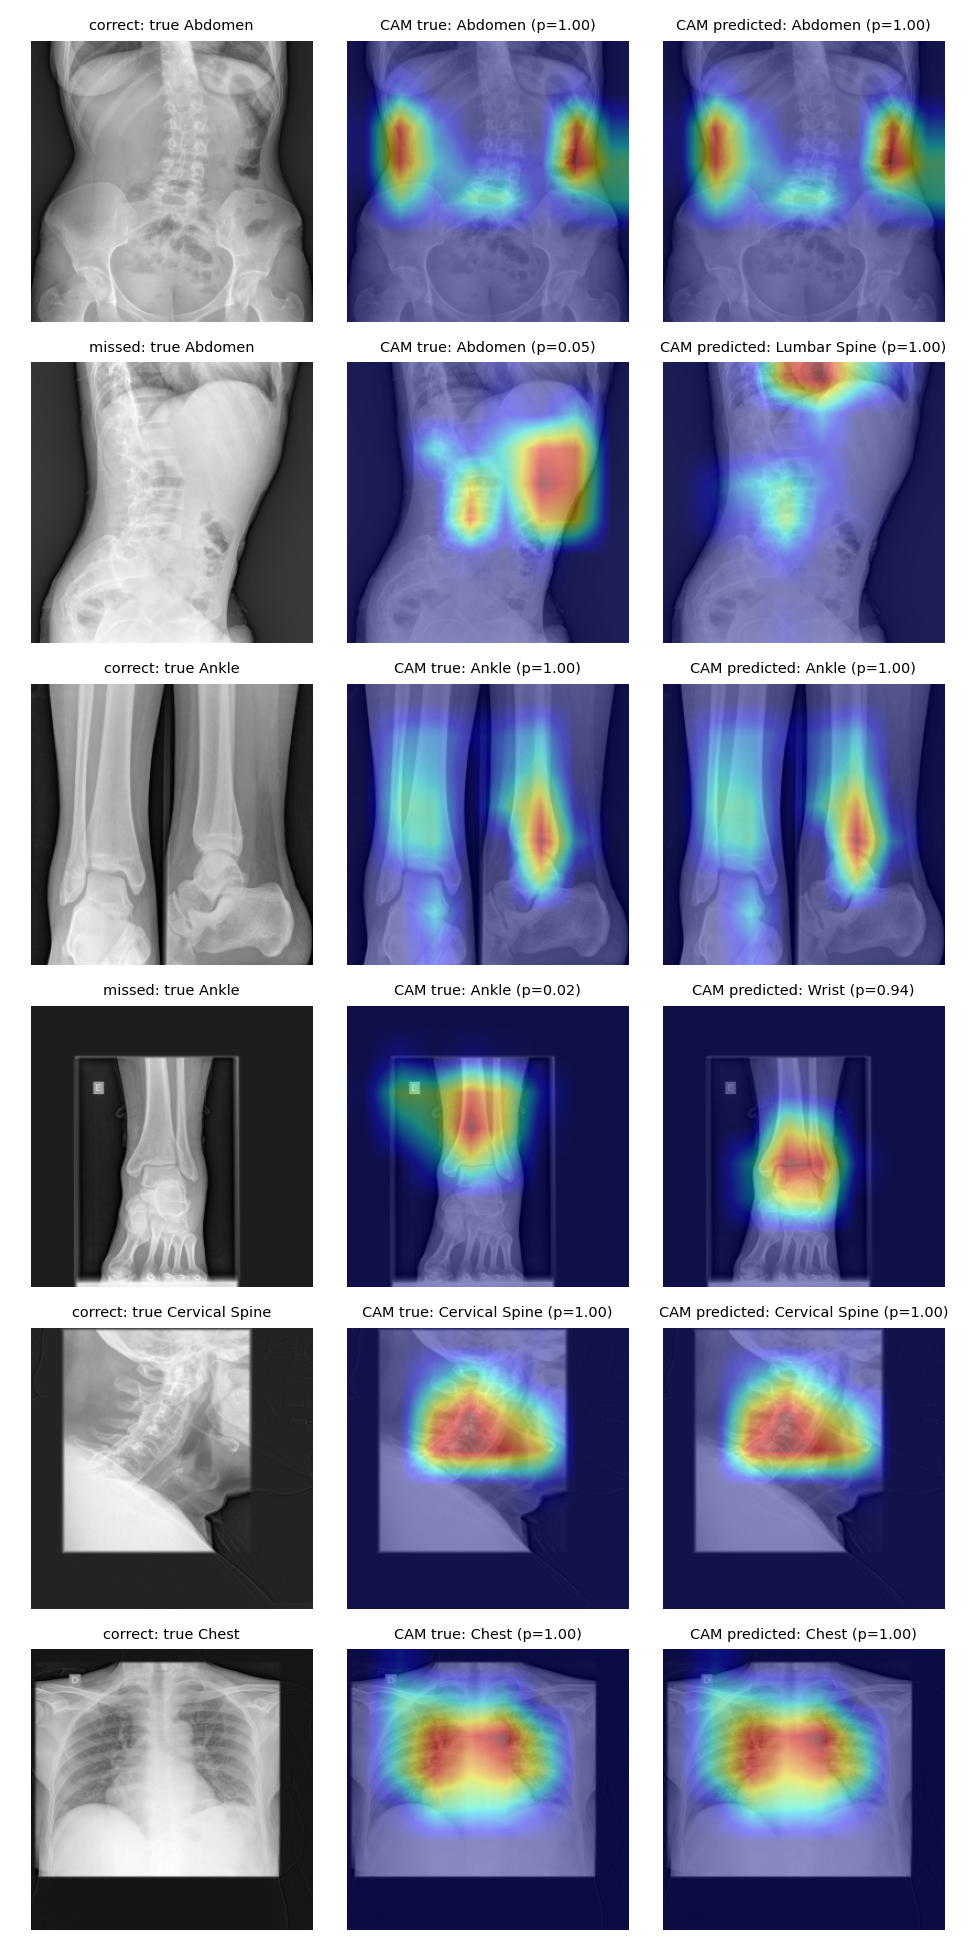
\includegraphics[width=0.325\textwidth]{gradcam_gallery_1.png}\hfill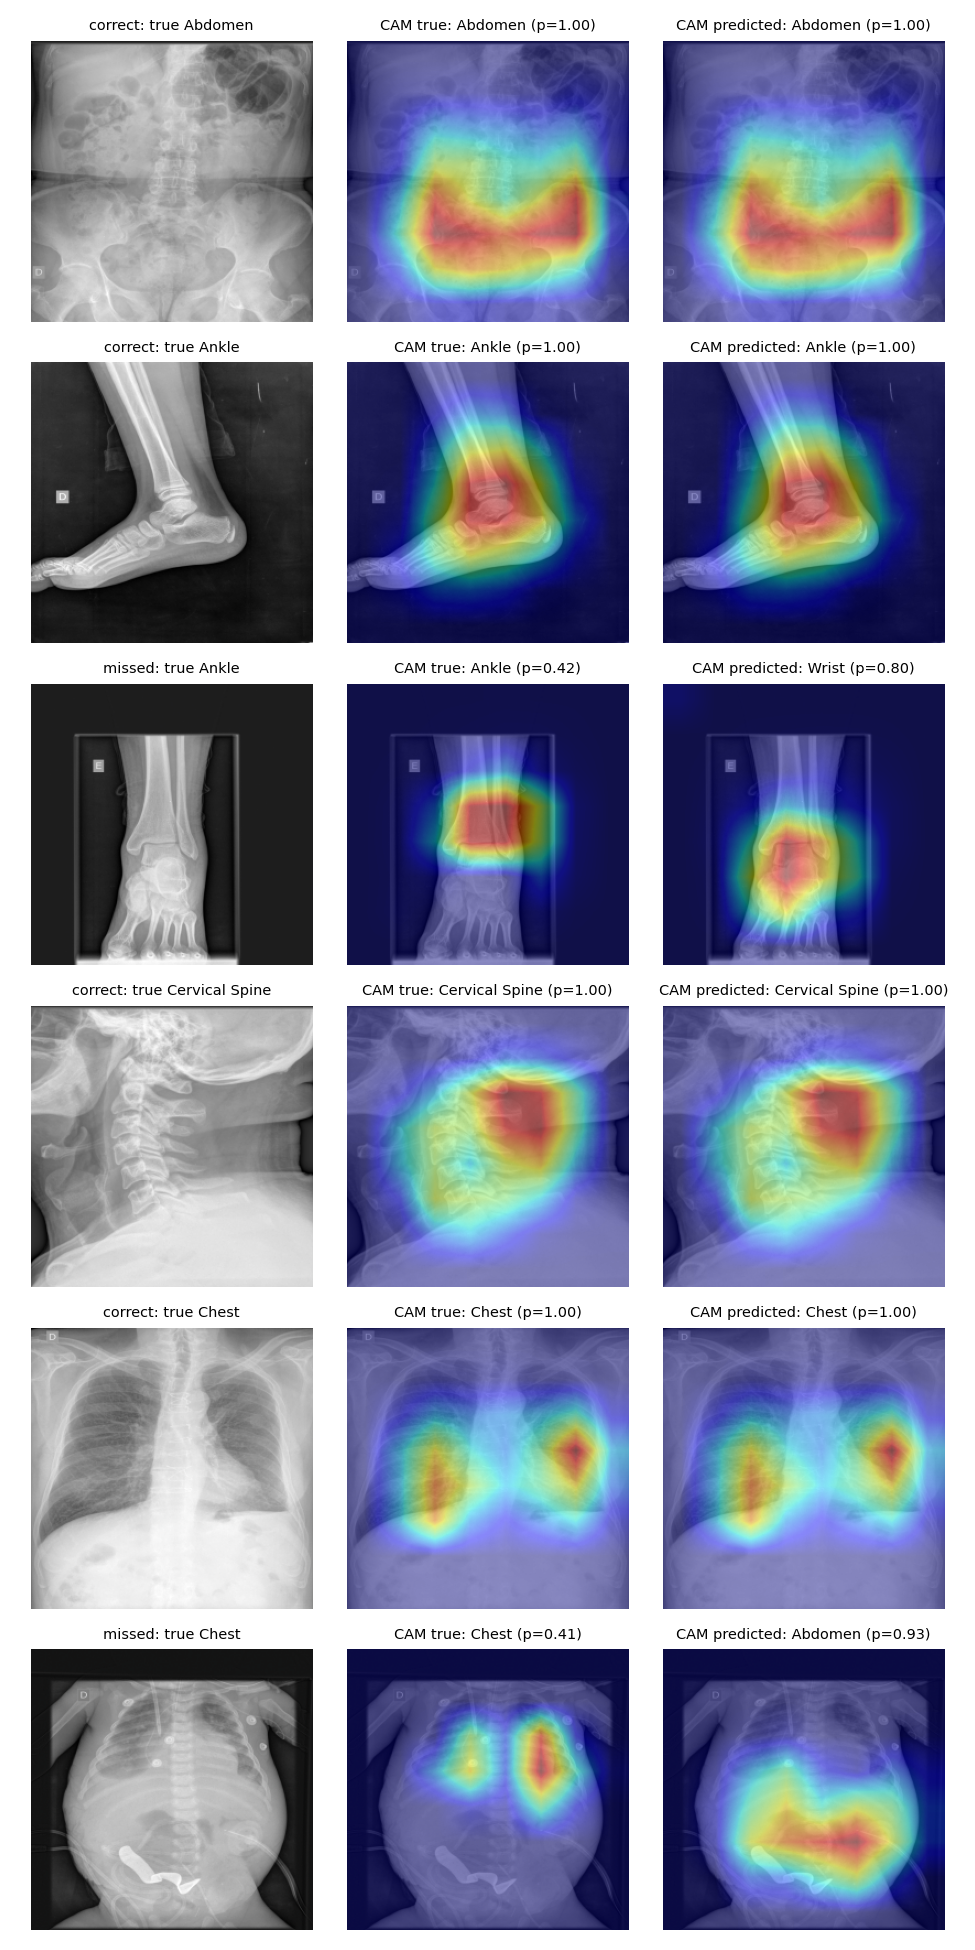
\includegraphics[width=0.325\textwidth]{gradcam_gallery_2.png}\hfill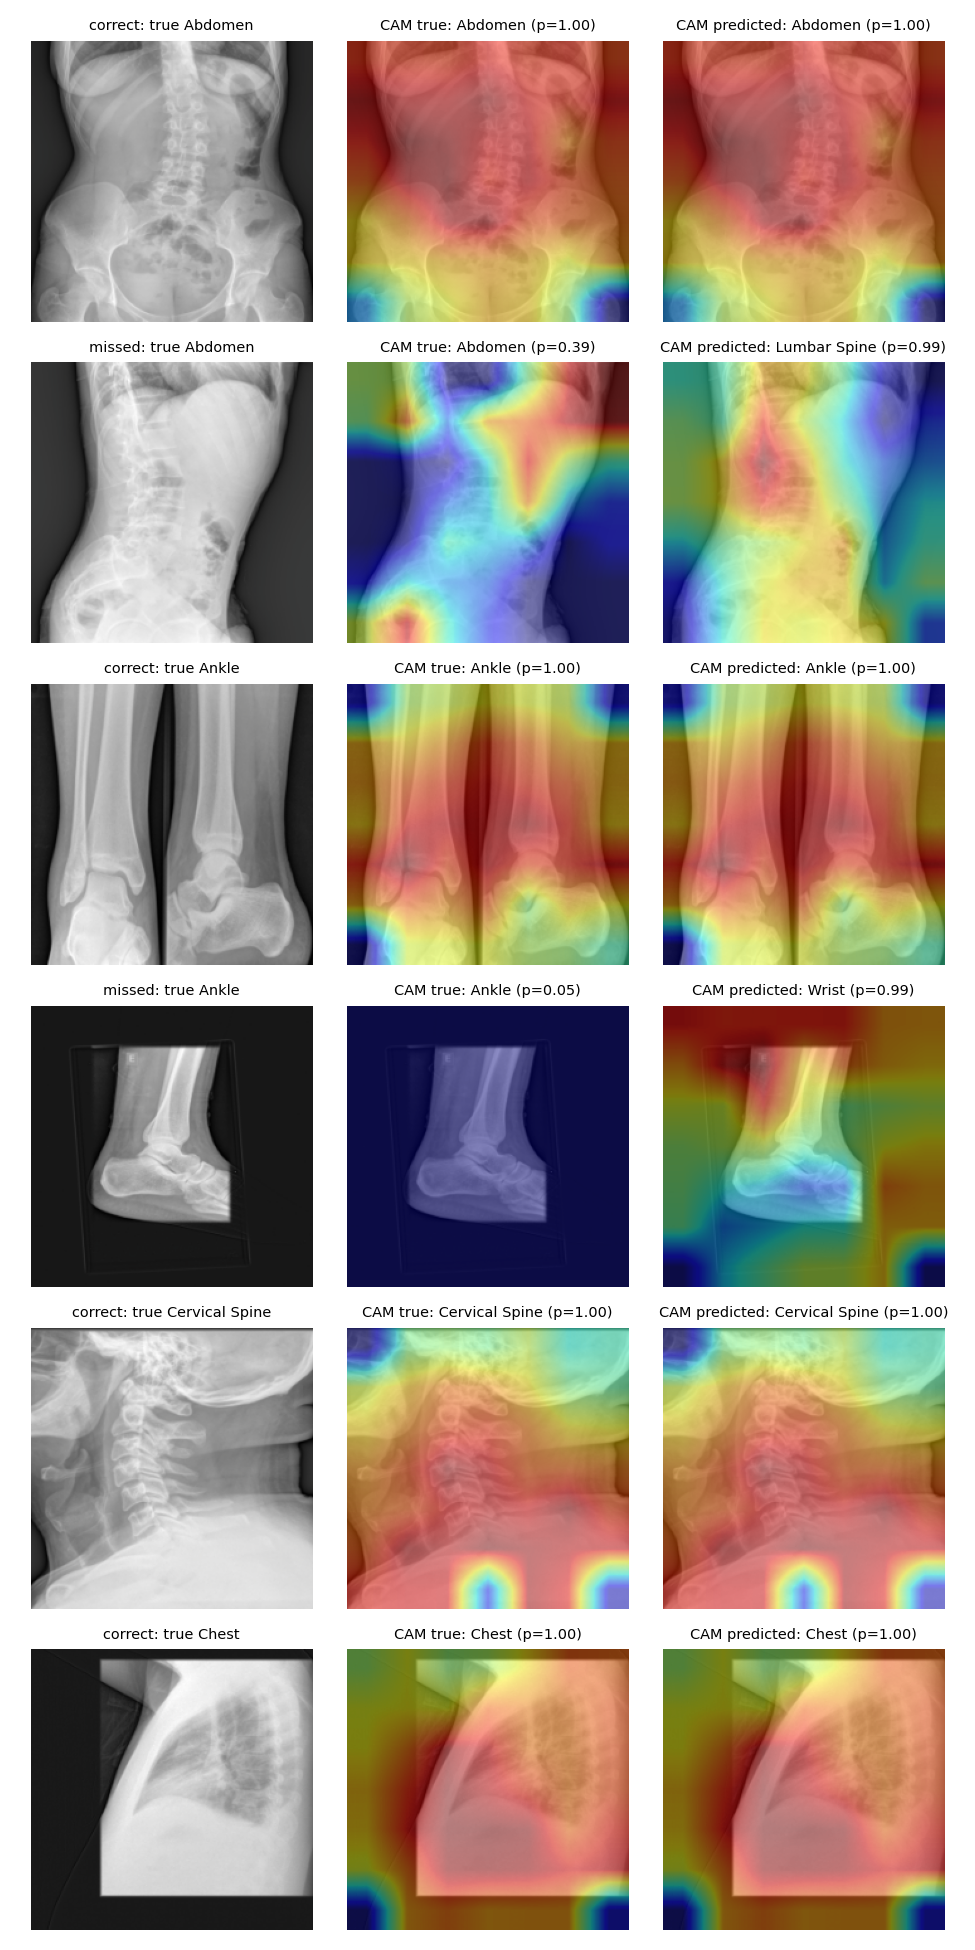
\includegraphics[width=0.325\textwidth]{gradcam_gallery_3.png}\caption{Grad-CAM galleries for ConvNeXt-T (left), ResNet50 (middle) and Swin-T (right). For each class there is one correct and one missed held-out image, with the map for the true class and for the predicted class.}\label{fig:13}\end{figure}\suppressfloats[t]




